%\documentclass[iop,revtex4]{emulateapj}% change onecolumn to iop for fancy, iop to twocolumn for manuscript
\documentclass[onecolumn]{emulateapj}% change onecolumn to iop for fancy, iop to onecolumn for manuscript
%\documentclass[preprint]{aastex}

%\usepackage{lineno}
%\usepackage{blindtext}
%\linenumbers

\let\pwiflocal=\iffalse \let\pwifjournal=\iffalse
%From: http://arxiv.org/format/1512.00483
%% For anyone who downloaded my source file from arxiv:
%% I stole most of this setup.tex from a paper by Peter .K.G. Williams, but I made a bunch of edits to satisfy my own needs. You might check his paper out (http://arxiv.org/abs/1409.4411) for the original source file or contact him if you have any questions, since I don't really understand how some of these things work. 
%One cool thing it does is you can define an object, just that when someone clicks on the pdf it will link to simbad. I could never quite get this to work, probably because you have to get the text exactly right and my motivation for getting it to work was not super high. 


% basic packages
\usepackage{amsmath,amssymb}
\usepackage[breaklinks,colorlinks,urlcolor=blue,citecolor=blue,linkcolor=blue]{hyperref}
\usepackage{epsfig}    
\usepackage{graphicx}    
\usepackage{lineno}
\usepackage{natbib}
\usepackage{bigints}
\usepackage[outdir=./]{epstopdf}



% font stuff
\usepackage[T1]{fontenc}
\pwifjournal\else
  \usepackage{microtype}
\fi


% emulateapj has overly conservative figure widths, I think because some
% people's figures don't have good margins. Override.
\pwifjournal\else
  \makeatletter
  \renewcommand\plotone[1]{%
    \centering \leavevmode \setlength{\plot@width}{0.95\linewidth}
    \includegraphics[width={\eps@scaling\plot@width}]{#1}%
  }%
  \makeatother
\fi


\makeatletter

\newcommand\@simpfx{http://simbad.u-strasbg.fr/simbad/sim-id?Ident=}

\newcommand\MakeObj[4][\@empty]{% [shortname]{ident}{url-escaped}{formalname}
  \pwifjournal%
    \expandafter\newcommand\csname pkgwobj@c@#2\endcsname[1]{\protect\object[#4]{##1}}%
  \else%
    \expandafter\newcommand\csname pkgwobj@c@#2\endcsname[1]{\href{\@simpfx #3}{##1}}%
  \fi%
  \expandafter\newcommand\csname pkgwobj@f#2\endcsname{#4}%
  \ifx\@empty#1%
    \expandafter\newcommand\csname pkgwobj@s#2\endcsname{#4}%
  \else%
    \expandafter\newcommand\csname pkgwobj@s#2\endcsname{#1}%
  \fi}%

\newcommand\MakeTrunc[2]{% {ident}{truncname}
  \expandafter\newcommand\csname pkgwobj@t#1\endcsname{#2}}%

\newcommand{\obj}[1]{%
  \expandafter\ifx\csname pkgwobj@c@#1\endcsname\relax%
    \textbf{[unknown object!]}%
  \else%
    \csname pkgwobj@c@#1\endcsname{\csname pkgwobj@s#1\endcsname}%
  \fi}
\newcommand{\objf}[1]{%
  \expandafter\ifx\csname pkgwobj@c@#1\endcsname\relax%
    \textbf{[unknown object!]}%
  \else%
    \csname pkgwobj@c@#1\endcsname{\csname pkgwobj@f#1\endcsname}%
  \fi}
\newcommand{\objt}[1]{%
  \expandafter\ifx\csname pkgwobj@c@#1\endcsname\relax%
    \textbf{[unknown object!]}%
  \else%
    \csname pkgwobj@c@#1\endcsname{\csname pkgwobj@t#1\endcsname}%
  \fi}

\makeatother


% Evil magic to patch natbib to only highlight the year paper refs, not the
% authors too; as seen in ApJ. From
% http://tex.stackexchange.com/questions/23227/.

\pwifjournal\else
  \usepackage{etoolbox}
  \makeatletter
  \patchcmd{\NAT@citex}
    {\@citea\NAT@hyper@{%
       \NAT@nmfmt{\NAT@nm}%
       \hyper@natlinkbreak{\NAT@aysep\NAT@spacechar}{\@citeb\@extra@b@citeb}%
       \NAT@date}}
    {\@citea\NAT@nmfmt{\NAT@nm}%
     \NAT@aysep\NAT@spacechar\NAT@hyper@{\NAT@date}}{}{}
  \patchcmd{\NAT@citex}
    {\@citea\NAT@hyper@{%
       \NAT@nmfmt{\NAT@nm}%
       \hyper@natlinkbreak{\NAT@spacechar\NAT@@open\if*#1*\else#1\NAT@spacechar\fi}%
         {\@citeb\@extra@b@citeb}%
       \NAT@date}}
    {\@citea\NAT@nmfmt{\NAT@nm}%
     \NAT@spacechar\NAT@@open\if*#1*\else#1\NAT@spacechar\fi\NAT@hyper@{\NAT@date}}
    {}{}
  \makeatother
\fi


% Object data
\MakeObj{n33370}{NLTT\%2033370}{NLTT~33370\,AB}
\MakeTrunc{n33370}{NLTT~33370}
\MakeObj{tvlm}{TVLM\%20513-46546}{TVLM~513--46546}

% utility

\newcommand{\vdag}{(v)^\dagger}
\newcommand{\oxygen}{O$_2$}
\newcommand{\water}{H$_2$O}
\newcommand{\kepler}{{\it Kepler}}
\newcommand{\logg}{$log~g$ }
\newcommand{\metal}{[M/H]}
\newcommand{\um}{$\mu$m}
\newcommand{\fbol}{$F_{\mathrm{bol}}$}
\newcommand{\mbol}{$m_{\mathrm{bol}}$}
\newcommand{\Mbol}{$M_{\mathrm{bol}}$}
\newcommand{\rapsq}{$R_{ap}^2$}
\newcommand{\rchisq}{$\chi^2_{\nu}$}
\newcommand{\hipp}{{\it Hipparcos}}


\newcommand\aafd{erg~s$^{-1}$~cm$^{-2}$~\AA$^{-1}$} % "AAngstrom flux density"
\newcommand\amlt{$\alpha_{\rm MLT}$} % convective mixing length parameter
\newcommand\apx{\ensuremath{\sim}}
\newcommand\cgsflux{erg~s$^{-1}$~cm$^{-2}$}
\newcommand\cgslum{erg~s$^{-1}$}
\newcommand\chandra{\textit{Chandra}}
\newcommand\citeeg[1]{\citep[\eg,][]{#1}}
\newcommand\cps{ct~s$^{-1}$}
\newcommand\dd{\ensuremath{\text{d}}}
\newcommand\eg{\textit{e.g.}}
\newcommand\etal{\textit{et~al.}}
\newcommand\ewha{\ensuremath{\text{EW}(\ha)}}
\newcommand\fig[1]{Figure~\ref{f.#1}}
\newcommand\ha{{\ensuremath{\text{H}\alpha}}}
\newcommand\I{\mathcal{I}}
\newcommand\ie{\textit{i.e.}}
\newcommand\kms{km~s$^{-1}$}
\newcommand\ls{L$_\odot$}
\newcommand\mj{M$_\text{J}$}
\newcommand\ms{M$_\odot$}
\newcommand\nupk{\ensuremath{\nu_\text{pk}}}
\newcommand\percc{cm$^{-3}$}
\newcommand\rcs{\ensuremath{\chi_r^2}}
\newcommand\rj{R$_\text{J}$}
\newcommand\sect[1]{Section~\ref{s.#1}}
\newcommand\sherpa{\textsf{Sherpa}}
\newcommand\sti{Stokes~$I$}
\newcommand\stiv{Stokes~$I$ and~$V$}
\newcommand\stv{Stokes~$V$}
\newcommand\swift{\textit{Swift}}
\newcommand\tb{\ensuremath{T_\text{b}}}
\newcommand\tbl[1]{Table~\ref{t.#1}}
\newcommand\teff{\ensuremath{T_\text{eff}}}
\newcommand\todo[1]{\textcolor{red}{#1}}
\newcommand\ujy{$\mu$Jy}
\newcommand\ujybm{$\mu$Jy~bm$^{-1}$}
\newcommand\uv{$u$\mbox{-}$v$}
\newcommand\vsi{\ensuremath{v \sin i}}

\newcommand\Lb{\ensuremath{L_\text{bol}}}
\newcommand\Lh{\ensuremath{L_\ha}}
\newcommand\Lr{\ensuremath{L_\text{R}}}
\newcommand\sLr{\ensuremath{L_{\nu,\text{R}}}}
\newcommand\Lu{\ensuremath{L_\text{UVW1}}}
\newcommand\Lx{\ensuremath{L_\text{X}}}
\newcommand\Lxf{\ensuremath{L_{\text{X},f}}}
\newcommand\Lxq{\ensuremath{L_{\text{X},q}}}
\newcommand\lb{\ensuremath{[\Lb]}}
\newcommand\lh{\ensuremath{[\Lh]}}
\newcommand\lr{\ensuremath{[\Lr]}}
\newcommand\slr{\ensuremath{[\sLr]}}
\newcommand\lu{\ensuremath{[\Lu]}}
\newcommand\lx{\ensuremath{[\Lx]}}
\newcommand\lxf{\ensuremath{[\Lxf]}}
\newcommand\lxq{\ensuremath{[\Lxq]}}
\newcommand\lhlb{\ensuremath{[\Lh/\Lb]}}
\newcommand\lrlb{\ensuremath{[\Lr/\Lb]}}
\newcommand\lulb{\ensuremath{[\Lu/\Lb]}}
\newcommand\lxlb{\ensuremath{[\Lx/\Lb]}}
\newcommand\lxflb{\ensuremath{[\Lxf/\Lb]}}
\newcommand\lxqlb{\ensuremath{[\Lxq/\Lb]}}
\newcommand\slrlb{\ensuremath{[\sLr/\Lb]}}
\newcommand\slrlx{\ensuremath{[\sLr/\Lx]}}
\newcommand\slrlxf{\ensuremath{[\sLr/\Lxf]}}
\newcommand\slrlxq{\ensuremath{[\sLr/\Lxq]}}


\providecommand{\eprint}[1]{\href{http://arxiv.org/abs/#1}{#1}}
\providecommand{\adsurl}[1]{\href{#1}{ADS}}
\newcommand{\name}{\emph{K2}}
\def\vsini{$v\sin{i_*}$}

\slugcomment{In preparation}

\shorttitle{\name \emph{K2} variability of YSOs}

\shortauthors{Gully-Santiago et al.}

\bibliographystyle{yahapj}

\begin{document}
 
\title{K2 variability of young stars towards Ophiuchus and Scorpius}

\author{Michael A. Gully-Santiago,\altaffilmark{1} Greg Herczeg,\altaffilmark{1} et al.}


\altaffiltext{1}{Kavli Institute for Astronomy and Astrophysics, Beijing, China}

\begin{abstract}
We present summary statistics of the variability of pre-main sequence stars observed towards Ophiuchus and Scorpius with high precision \emph{K2} photometric monitoring.
\end{abstract}

\keywords{stars: fundamental parameters --- stars: individual (\name) ---  stars: low-mass -- stars: statistics}

\maketitle

\section{Introduction}\label{sec:intro}

Pre-main sequence stars vary more than their main sequence star counterparts.  Young stars have disks \citep{2011ARA&A..49...67W}.

In young stars we expect two types of time-variability: flares and rotationally induced sinusoidal variability attributable to longitudinally assymetric starspots coming into and out of view.  Flares occur from accretion events and other phenomena, and have a relatively short time scale of minutes Davenport et al. XX.  The starspot rotational variability has typically a much lower amplitude than the flares, and has periods of typically a few days.

\section{Observations}\label{sec:obs} 
\emph{K2} observed \emph{Ophiuchus} and \emph{Scorpius} in cycle 2 in 2014.  We assembled a sample of 1678 sources that were targeted as known young cluster members or candidate young stars by \emph{K2} proposals XX-YY.  We acquired long candence lightcurves for this sample, along with about 2000 other sources from cycle 2 that were targeted for reasons other than being candidate young stars.  We refer to these samples as the YSO sample and control samples, respectively.

We used the data available from MAST, which were reduced following the method of Vanderburg \& Johnson XX.  These lightcurves have been de-trended from their raw signal, but some lightcurves still exhibit large instrumental artifacts.  The largest artifact is approximately half-way through the XX day observation window.  All lightcurves have a gap in this time, and some have discontinuous relative fluxes directly before and after this gap.

\section{Analysis}
We computed the standard deviation $\sigma$ and inter-quartile range $Q_3-Q_1$ for each lightcurve.  Twenty of the 1678 sources were dropped for having undefined standard deviation values, probably due to an errant pixel value.  Our YSO sample was reduced to 1658.  The standard deviation and interquartile range contain information about the average variability of the lightcurve.  The interquartile range is robust against large deviations that occur over a short timescale, with short defined as affecting less than 25\% of the time samples.

The standard deviation, on the other hand, is much more sensitive to outlying data points, which are weighted as the square of the difference from the mean.  So in a plot of standard deviation versus interquartile range, we expect flares and starspot-induced variability to be separable.  We constructed a plot of $\log{\sigma}$ versus $\log{IQR}$, shown in Figure \ref{fig:k2_overview}.

\begin{figure*}
	\centering
	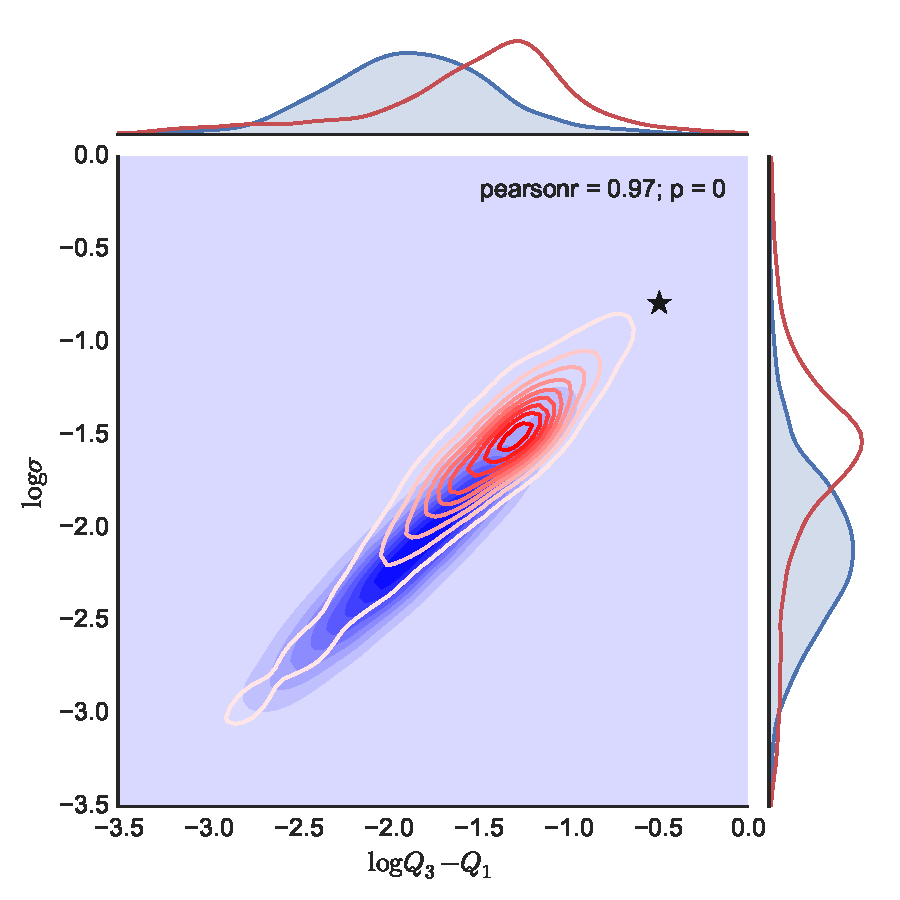
\includegraphics[width=0.95\textwidth]{figures/K2_YSO_variability_overview.pdf} 
	\caption{Variability of \emph{K2} cycle 2 light curves of young stars or candidate young stars towards Ophiuchus and Scorpius.  The standard devation scales linearly with the interquartile range for sources with little or no flare events.  Stars with high flare amplitude and/or high number of flares will exhibit large deviations from the linear trend.  Perfectly sinusoidal lightcurves will follow the dashed line.  }
	\label{fig:k2_overview}
\end{figure*}


\acknowledgements
ADS and Astropy.

{\it Facilities:} \facility{Smith (IGRINS)}

\clearpage

\bibliographystyle{apj}
\bibliography{ms}

\end{document}
